% ============================================
%  Article Class (This is a LaTeX2e document)
% ============================================
\documentclass[12pt]{scrartcl}

\usepackage[english]{babel}
\usepackage[utf8]{inputenc}

\usepackage{enumitem}
\usepackage[round]{natbib}
\usepackage{color}

\newcommand\reft[3][]{#2~\ref{#3}#1}
\newcommand\refp[3][]{(#2~\ref{#3}#1)}
\newcommand\refsect[1]{\reft{Section}{#1}}
\newcommand\refsecp[1]{\refp{Sec.}{#1}}
\newcommand\reftabt[1]{\reft{Table}{#1}}
\newcommand\reftabp[1]{\refp{Tab.}{#1}}

% ======
%  Math
% ======
\usepackage{amsmath}
\usepackage{amsthm}
\usepackage{mathtools} % \mathclap
\newtheorem{thm}{Theorem}[section]
\newtheorem{cor}[thm]{Corollary}
\newtheorem{lem}[thm]{Lemma}
\newtheorem{prop}[thm]{Proposition}
\newtheorem{property}[thm]{Property}
\theoremstyle{definition}
\newtheorem{defn}[thm]{Definition}
\newtheorem{assum}[thm]{Assumption}
\theoremstyle{remark}
\newtheorem{rem}[thm]{Remarque}
\numberwithin{equation}{section}

\usepackage{amssymb}
\newcommand{\prob}[1]{\mathbb{P}\left(#1\right)}
\newcommand{\Ker}[1]{\mathrm{Ker}\left(#1\right)}
\newcommand{\Image}[1]{\mathrm{Im}\left(#1\right)}
\newcommand{\diag}[1]{\mathrm{diag}\left(#1\right)}
\newcommand{\Vect}[1]{\mathrm{Vect}\left\{#1\right\}}

% ============================
%  Figures and relative paths
% ============================
\usepackage{graphicx}
\graphicspath{{figures/}}
\usepackage{import}
\makeatletter
  \def\relativepath{\import@path}
\makeatother
\newcommand\reffigt[2][]{\reft[#1]{Figure}{#2}}
\newcommand\reffigp[2][]{\refp[#1]{Fig.}{#2}}

% ==========
%  Document
% ==========
\begin{document}

\title{rba.core\\ Building constraint matrices from RBA data.}%
\author{Biosys - MAIAGE}%
\date{\today}%

\maketitle

\newpage

\tableofcontents

\newpage

\section{Overview of RBA constraints}

In order to build an RBA system, we need to build three sets of constraints.

\begin{itemize}
  \item[($C_1$)] Mass conservation.
  \item[($C_2$)] Capacity constraints for enzymes and process machines, e.g., ribosomes.
  \item[($C_3$)] Density constraints.
\end{itemize}

All these constraints are linear (in)equalities.
We will write them in matrix form, as it is the best way to summarize
all information needed to build a constraint.

\subsection{Important concepts and conventions}

\paragraph{Production/degradation vector for macromolecules}
In the following, each macromolecule is described by its \textbf{production vector}.
It is a column vector containing the metabolites necessary to build it,
with a \textbf{minus} sign for metabolites consumed and a \textbf{plus} sign for byproducts generated.
Similarly, we define \textbf{degradation vectors}.

\paragraph{Concentration to flux conversion}
Suppose you have a metabolite at concentration $C = n/V$.
At growth-rate $\mu$, we have $dV \simeq \mu V$.
The variation of concentration due to dilution is
\[
  dC = d(n/V) = -n/V^2 dV = -\mu C
\]
In other words, in order to keep the concentration constant,
we need an input metabolite flux of
\[
  \nu = \mu C
\]
When a variable is expressed as a concentration, it may be necessary to
convert it to a flux by using this relationship.
When necessary, we indicate this conversion by inserting a conversion
matrix between the main matrix and the variable vector.

\paragraph{Variable representation}
When we go to full matrix representation in the figures,
variables are represented as a single row vector below matrices.
This convention clarifies how columns and variables are associated.
Note the transpose at the end of the row vector if you are worried about
mathematical purity.

\subsection{Variables}

RBA uses 4 sets of variables:

\begin{itemize}
  \item $\nu = (\nu_1, \ldots ,\nu_R)$: Fluxes through metabolic reactions,
  where $R$ is the number of reactions.
  \item $E = (e_1, \ldots, e_E)$: Enzyme concentrations,
  where $E$ is the number of enzymes.
  \item $P = (p_1, \ldots, p_P)$: Process machine concentrations,
  where $P$ is the number of processes.
  \item $T = (t_1, \ldots, t_T) = (TF, TC)$:
  Target values, where $T$ is the number of targets.
  Targets may be expressed as fluxes or concentrations.
  We note target fluxes $TF$ and target concentrations $TC$.
  When necessary, we assume that flux targets are all listed first,
  i.e., $T = (TF, TC)$.

\end{itemize}
Targets are production/degradation requirements for the cell to be fully functional
(e.g. keeping key metabolites at some given concentration,
producing housekeeping proteins, producing/degrading mRNAs).
Note that target values may actually be predetermined constant values,
while all others are true variables that must be optimized.
We will see later how predetermined constant values may be eliminated.

\subsection{Mathematical formulation of RBA constraints}

Before we group all constraints and variables into a single matrix,
here is an overview of the 3 family of constraints used in RBA models.

\paragraph{$(C_1)$ Mass conservation}

\[
\overbrace
{
\underbracket{S\nu}_{\parbox{2cm}{\scriptsize metabolic flux generated by metabolism}}
+
\underbracket{\mu C_E E + \mu C_P P}_{\parbox{3cm}{\scriptsize precursors used/byproducts generated by producing new molecules}}
}^{\text{\normalsize `Variable' terms}}
+
\overbrace
{
\underbracket{\mu C_{TC} TC + C_{TF}TF}_{\parbox{3cm}{\scriptsize precursors used/byproducts generated by producing new molecules}}
}^{\text{\normalsize Constant terms}} \\
=0
\]

where $S$ is the stoichiometry matrix of the metabolism,
with metabolites as rows and reactions as columns.
$C_.$ are composition matrices where every column is the composition of
one of the molecules, e.g. $(C_E)_i$ is the composition of the $i$th enzyme
(see definition of composition vector above).
Note the usage of $\mu$ along with $E$, $P$ and $TC$ as way of converting
concentrations into fluxes.

\paragraph{$(C_2)$ Capacity constraints}

\[
\diag{k_E^{backward}} E \leq \nu \leq \diag{k_E^{forward}} E
\]

where $k_E^{backward}$ is a vector containing the backward catalytic constants of enzymes.

\[
\mu MC_E E + \mu MC_P P + \mu MC_{TC} TC + MC_{TF} TF \leq \diag{k_P} P
\]

where $k_P$ is a vector containing the capacities of process machines.
$MC_.$ are matrices containing machine costs to produce macromolecules,
e.g. $(MC_E)_{ij}$ quantifies how much the machine from the $i$th process is needed
to build the $j$th enzyme.
For example, the ribosome (machine of translation process) has a processing
capacity of $k_P \simeq 72,000$ amino acid per hour.
If an enzyme contains 3 proteins of $300$ amino acid each, its machine cost
is $MC = 900$.

\paragraph{$(C_3)$ Density constraints}

\[
W_E E + W_P P + W_{TC} TC \leq \overline{D}
\]
where $W_.$ are weight matrices,
e.g. $(W_E)_{ij}$ is the weight of the $j$th enzyme in the $i$th compartement.
$\overline{D}$ is a vector containing the maximal weight per compartement,
e.g. $D_i$ is the maximum weight in the $i$th compartment.



\section{Constraint matrices}

\subsection{Mass conservation ($C_1$)}

The mass conservation constraint is represented by a matrix where rows
are metabolites, labelled $M = (m_1, \ldots, m_M)$.
Metabolite fluxes must cancel out in order to achive mass conservation.
Note that numerous variables are expressed as concentrations and must be
converted to fluxes as explained previously.

\reffigt{fig:mass_conservation} shows how mass conservation is expressed
in matrix formalism.
The main matrix contains the metabolic reactions,
the production vectors for catalytic elements,
the production/degradation vectors for target elements.
This matrix is growth-rate independent.
The second matrix converts variables that are expressed as
concentrations to fluxes.
This can also be seen as multiplying the appropriate columns in the main matrix
by the growth-rate.

\begin{figure}
  \centering
  \includegraphics[width=\linewidth]{mass_conservation}
  \caption{Mass conservation constraint.
  Bars in the main matrix are metabolic reaction or
  production/degradation vectors associated with each variable.}
  \label{fig:mass_conservation}
\end{figure}

\subsection{Capacity constraints ($C_2$)}

The capacity constraintes are represented by a matrix where rows are enzymes
or process machineries.
Currently, we use two different formalisms for enzymes and process machineries.

Enzymes are associated to exactly one reaction that may be reversible.
For every enzyme we have the following constraint:
\[
  \nu \leq k_{forward} e_i
\]
where $\nu$ is the flux through the reaction catalyzed by $e_i$.
If the reaction is irreversible, we have the additional constraint
\[
  \nu \geq -k_{backward} e_i
\]
In order to write all constraints, we need a reaction to enzyme mapping.
This is represented by a matrix where we have one row per constraint.
Each row has a 1 on the column corresponding to the reaction catalyzed,
and 0s everywhere else.

Process machineries participate in the synthesis/degradation of several
macromolecules (enzymes, machineries and targets).
For every target, we have a constraint of the form
\[
   [machinery\_cost].[E, P, T]^T \leq k_{machinery} p_i
\]
Every macromolecule has a set of machinery costs associated with it.
It tells how much a machinery is used in order to produce/degrade the
macromolecule (the cost is often 0).

The final matrices are very sparse \reffigp{fig:capacity_constraints}.
A first matrix contains the reaction to enzyme mapping and the machinery
costs. This matrix is growth-rate independent.
A second matrix contains efficiencies, that may depend on growth-rate.
Note that we did not need to convert concentrations to fluxes here.

\begin{figure}
  \centering
  \includegraphics[width=\linewidth]{capacity_constraints}
  \caption{Capacity constraints.}
  \label{fig:capacity_constraints}
\end{figure}

\subsection{Density constraints ($C_3$)}

Density constraints are represented by matrices where rows are compartments,
labelled $C = (c_1, \ldots, c_C)$.

Every variable that represents a concentration participates to this constraint.
For every macromolecule, we define a weight vector that defines how much
volume one molecule occupies in every compartment (in user defined units).
By putting these vectors together we get a weight matrix.

The user also defines a vector of maximal weights for every compartment,
yielding a simple set of constraints \reffigp{fig:density_constraints}.
Only the right-hand part may contain growth-rate dependent values.
Again, no conversion from concentration to flux is needed here.

\begin{figure}
  \centering
  \includegraphics[width=\linewidth]{density_constraints}
  \caption{Density constraints.}
  \label{fig:density_constraints}
\end{figure}

\clearpage

\section{Building matrices from XML files}

In this file, we briefly describe how matrices are built from files.

\paragraph{Building blocks}
\reffigt{fig:blocks} shows the blocks that are used to build the final matrices.
\begin{figure}
  \centering
  \includegraphics[width=\linewidth]{blocks}
  \caption{Blocks that need to be assembled.
  There is also a vector of constraint signs that is omitted here
  (E for equality, L for lower than, G for greater than).}
  \label{fig:blocks}
\end{figure}

\paragraph{Stoichiometry matrix}
The stoichiometry matrix is built from metabolic reactions.
External metabolites are removed from the metabolite pool.

\paragraph{Density limits}
Density limits are simply extracted from RBADensity and assembled into a vector (one coefficient per compartment).

\paragraph{Species matrices}
\reffigt{fig:species_matrices} shows how macromolecules are broken down
into matrices describing their composition, machinery cost and weight.
In the end, they are merged into a single matrix describing composition,
machinery cost and weight of all metabolites and macromolecules.
\begin{figure}
  \centering
  \includegraphics[width=\linewidth]{species_matrices}
  \caption{Matrices extracted from macromolecule information.
  An example is given with proteins but in the end,
  they contain all macromolecules and all internal metabolites.}
  \label{fig:species_matrices}
\end{figure}

\paragraph{Enzyme and machinery matrices}
\reffigt{fig:machinery_matrices} shows how enzyme and process machinery matrices are built.
\begin{figure}
  \centering
  \includegraphics[width=\linewidth]{machinery_matrices}
  \caption{Every machinery can be described by a reaction matrix.
  Reactants are species (metabolites or macromolecules) needed to build the machinery
  and products are byproducts of the assembly process.
  Through matrix multiplication with the species matrices,
  we can deduce its composition, weight and machinery cost.}
  \label{fig:machinery_matrices}
\end{figure}

\paragraph{Target matrices}
Targets are either metabolites or macromolecules.
Their composition, machinery cost and weight can be extracted as columns from the species matrices.

\clearpage

\newpage
\appendix
\section{Eliminating target variables}

In the previous sections, we included all targets as variables.
In practice, most variables are predetermined, e.g., the target for
concentrations for metabolites is known, it does not need to be optimized.
Optimization algorithms will typically eliminate all such variables in a
presolving step, but we might want to eliminate them manually in order to
reduce matrix sizes.

The procedure is fairly simple: we extract the submatrix corresponding to
targets with known values, multiply it by the value vector, and move it
to the right-hand side~\reffigp{fig:target_elimination}.

\begin{figure}
  \centering
  \includegraphics{target_elimination}
  \caption{Procedure to reduce matrix size by eliminating targets
  with predefined values.
  This yield a smaller A matrix and a slightly more complicated b matrix.}
  \label{fig:target_elimination}
\end{figure}

%\clearpage

%
\section{Work in progress}

\subsection{Harmonize enzymes and process machineries}

Currently every reaction must be catalyzed by a different enzyme.
In comparison, process machineries, such as ribosomes, may catalyze multiple
production reactions.
We may use a similar system for enzymes where one enzyme may catalyze several
reactions.

In this case, the reaction to enzyme mapping becomes a little more complicated
and must take into account
\begin{itemize}
  \item Different k\_cat values for different reactions.
  \item Distinguish forward and backward reactions.
\end{itemize}
A side document explains how enzyme capacity constraints may be rewritten
in order to be closer to process capacity constraints.

Implementing the new mapping yields smaller matrices, as we need less
constraints overall.

\subsection{Matrix conditioning and objective function}

Performance is extremely variable because our matrix is not well conditioned.
Sometimes, adding zero rows and columns drastically improves convergence
(not sure why, cplex eliminates these rows and columns during presolving, but
somehow converges in fewer iterations, maybe a bigger matrix increases
convergence tolerance?).
Finding a good matrix scaling and objective function may affect performance
significantly.


%\bibliographystyle{myplainnat}
%\bibliography{biblio}

\end{document}
% ----------------------------------------------------------------
